\documentclass[a4j,10pt,dvipdfmx]{jarticle}
\usepackage{url}
\usepackage[version=3]{mhchem}
\usepackage{siunitx}
\usepackage[dvipdfmx]{graphicx}
\begin{document}
\section{10分間テスト}
 1) $1s^22s^22p^63s^23p^6$
 2) 2.11eV
  \section{実験の目的}
  量子化学計算ソフトを用いて,原子軌道の概念について学ぶ.
  
  加えてシアニン色素の紫外線吸収スペクトルを測定し,色素の色,吸収波長,分子構造における関係を調べる.

  シアニン色素のモデル分子の計算を行い,分子軌道と吸収の関係を考察する.

  \section{実験の原理}
  \subsection{原子軌道}
  原子にはK,L,M,N殻の電子殻が存在し,いくつかの原子軌道で構成されている.原子軌道は主量子数$n$,方位量子数$l$,磁気量子数$m$の組み合わせで区別される.
  $n=1,2,3...$,$l= 0,1,2,3,...,n-1$,$m=0,\pm1,\pm2,\pm3,...,\pm{l}$の組み合わせに対して軌道が対応する.


  \subsection{吸収スペクトル}
  物体の色は太陽光や電灯の光が物体に当たったときに、物体に特定の波長の光が吸収され,残りの光が反射されたものである.可視光はおよそ波長400nmから800nmの電磁波であり,波長の短いものは紫,長いものは赤に見える.
  白色光は可視光の領域が全部混じったものである.白色光のうちの一部は,補色関係にあり,吸収される色によってその補色関係を調べることができる.
  このような電子推移を利用した分析法が紫外可視分光法と呼ばれ,得た値が吸収スペクトルとなる.
  \subsection{分子軌道法}
  以下MO法とき記す.MO法は物質の電子状態を理解し,その性質や反応性を解明し,予測できるようにする方法である.MO法では分子に分布する複数のMOを計算で求める.
  分子に含まれる電子は,エネルギーの低いMOから順に配置される.電子に占有されて最もエネルギーの高い軌道をHOMO,電子に専有されてない最もエネルギーの低い軌道をLUMOと呼ぶ.

  ある分子に対して特定のエネルギーを持った光を照射すると,光を吸収し電子遷移が起こる.MOはシュレディンガーの波動方程式に当てはめ求めることができる.
  \section{実験手順}
  実験ではSpartranという分子軌道計算ソフトウェアを利用した.また紫外線吸収スペクトルの測定は日立ハイテクU5100型を用いた.
  \subsection{アルゴン原子の原子軌道の計算}
  \begin{enumerate}
    \item Spartranでアルゴン原子の原子軌道を計算した
    \item 原子軌道のエネルギーを表にまとめた
    \item K,L,M殻に属する原子軌道を図示した
  \end{enumerate}
  \subsection{シアニン色素の紫外線吸収スペクトルの測定}
  \begin{enumerate}
    \item 青のラベルの未知試料をセルに8割入れた
    \item セルを装置にセットし,紫外線吸収スペクトルを測定した
  \end{enumerate}
  \subsection{シアニン色素モデル分子の分子軌道計算}
  \begin{enumerate}
    \item シアニン色素$D_0~D_3$について吸収極大の波長と電子遷移に必要なエネルギーを求めた.
    \item シアニン色素$M_0~M_3$についてHOMOとLUMOそれぞれのエネルギーの差を求めた.
  \end{enumerate}
  \section{結果}
  \subsection{アルゴン原子の原子軌道}
  各軌道の概形をスケッチしたものをアルゴン原子の原子軌道の図として巻末に加えた.
  大きさは書いてあるとおりであり1番が一番小さく2から5番までが同じ大きさ,6から9までが一回り大きい同じ大きさだった.
  それぞれのエネルギーを表にまとめた.
  \begin{center}
    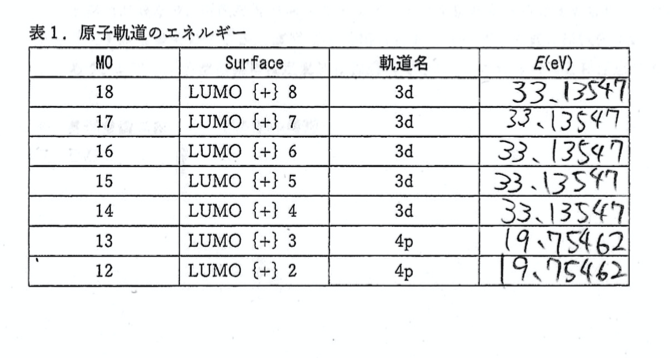
\includegraphics[width=15cm]{energy1.png}
  \end{center}
  \begin{center}
    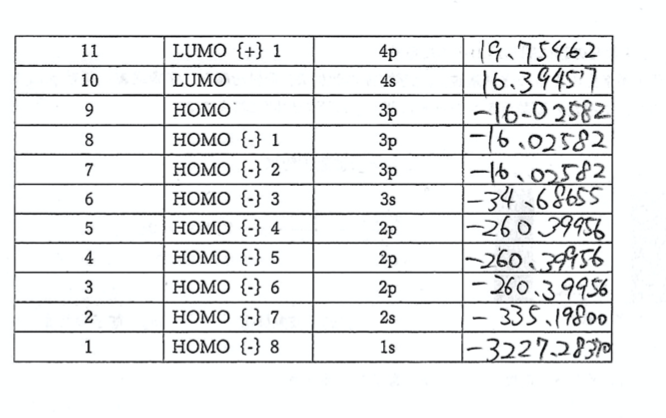
\includegraphics[width=15cm]{energy2.png}
  \end{center}
  スケッチの番号と対応している.
  \subsection{シアニン色素の紫外線吸収スペクトルの測定}

  レポートの結果と参考資料を巻末に加えた.
  この結果と資料を比べると測定した未知試料は$D_2$と推測できた.
  \subsection{シアニン色素モデル分子の分子軌道計算}
  シアニン色素$D_0~D_3$について吸収極大の波長と電子遷移に必要なエネルギーを表にまとめ下記のとおりとなった.
  \begin{center}
    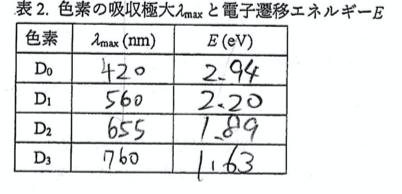
\includegraphics[width=15cm]{2.png}
  \end{center}

  シアニン色素$M_0~M_3$についてHOMOとLUMOそれぞれのエネルギーの差を表にまとめ下記のとおりとなった.
  \begin{center}
    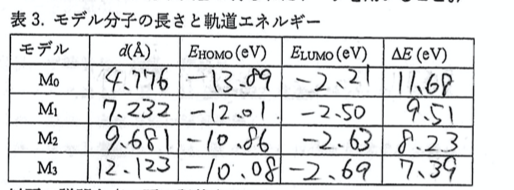
\includegraphics[width=15cm]{3.png}
  \end{center}
  \section{考察}
  \subsection{アルゴン原子の原子軌道}
  スケッチから2p軌道は$2p_x$,$2p_y$,$2p_z$,3p軌道は$3p_x$,$3p_y$,$3p_z$と方向の異なる同じ形をしている事がわかる.
  また原子軌道のエネルギーの大きさは$1s<2s<2p_x=2p_y=2p_z<3s<3p_x=3p_y=3p_z<4s<4p_x=4p_y<4p_z$...という序列と実際に一致していることが確認できた.


  シアニン色素の紫外線吸収スペクトルの測定結果とそこから計算した電子遷移エネルギーとシアニン色素モデル分子の分子軌道計算で出した電子遷移エネルギーは$D_2$は完全に一致する結果となった.
  一方でLUMOとHOMOの差のエネルギーは電子遷移エネルギーと一致しないのでLUMOとHOMOの間での遷移の結果ではない事がわかった.
  モデル分子の長さが大きくなるほどエネルギーは小さくなり波長は大きくなることがわかった.
  \section{感想}
  シアニン色素の紫外線吸収スペクトルの測定結果とソフトウェアで計算した結果が完全に一致していたので日立ハイテクU5100型はとても精密に測定できるのだと思った.
  \begin{thebibliography}{9}
    \bibitem{a} 電気通信大学『基礎科学実験』2021年,p60$\sim$70
  \end{thebibliography}
\end{document}
